%%%%%%%%%%%%%%%%%%%%%%%%%%%%%%%%%%%%%%%%%%%%%%%%%%%%%%%%%%%%%%%%%%%%%%%%
%
%     Curso   :   Analisis Aplicado I.
%     semestre:   otonyo de 1999

%%%%%%%%%%%%%%%%%%%%%%%%%%%%%%%%%%%%%%%%%%%%%%%%%%%%%%%%%%%%%%%%%%%%%%%%
\documentclass[12pt]{article}
\usepackage{latexsym}
\usepackage{lipsum}
\usepackage{graphicx}
\usepackage{float}
\usepackage{mathtools}
\usepackage{framed}
\usepackage[margin=1in]{geometry} 
\usepackage{amsmath,amsthm,amssymb}
\usepackage{caption}

\setlength\parindent{24pt}
\textwidth     =  6.5in
\textheight    =  8.2in
\oddsidemargin =  -0.2in
\topmargin     = -0.4in
%%%%%%%%%%%%%%%%%%%%%%%%%%%%%%%%%%%%%%%%%%%%%%%%%%%%%%%%%%%%%%%%%%%%%%%%
\newcommand{\ul}{\underline}
\begin{document}
\title{An\'alisis aplicado \\ {\small\tt Proyecto: m\'etodo de m\'aximo descenso}}
\author{Guillermo Santiago Novoa P\'erez   \\ {\small 000125089}}
\date{2 de febrero, 2015.}
\maketitle


\subsubsection*{{\large Objetivo}}

El proyecto tiene como finalidad estudiar el comportamiento te\'orico y pr\'actico del m\'etodo de m\'aximo descenso con b\'usqueda lineal exacta. En este punto es importante recordar que todos los m\'etodos estudiados en el curso est\'an guiados por las propiedades de la direcci\'on opuesta al gradiente. Por lo tanto, resulta fundamental comprender el funcionamiento de dicho m\'etodo en las funciones no lineales m\'as elementales:  las cuadr\'aticas estrictamente convexas.

 \begin{enumerate}
  \item  Las cuadr\'aticas que vamos a utilizar en el proyecto son de la forma
  \[
      f(x) =  \frac{1}{2} x^T Hx  + g^Tx
  \]
  en donde $H$ es una matriz sim\'etrica positiva definida de $n \times n$ con n\'umero de condici\'on conocido; el vector $g$ es generado en forma aleatoria con la funci\'on {\tt randn}.  
  
 \item El resultado sobre la convergencia global se formula como sigue:
 
       \begin{quotation}
 
        {\bf Teorema:}  El m\'etodo de m\'aximo descenso aplicado a cuadr\'�ticas estrictamente convexas satisface la siguiente propiedad
        \begin{eqnarray}  \label{desigualdad}
           ||x_{k+1} - x^* ||_H^2 \le \left [   \frac{ \lambda_{\rm max} - \lambda_{\rm min} }{ \lambda_{\rm max} + \lambda_{\rm min} } \right ]^2
           ||x_{k} - x^* ||_H^2,
        \end{eqnarray}
        \end{quotation}
        
      \noindent  en donde $|| \cdot ||_H$ representa a la norma vectorial inducida por $H$; $\lambda_{\rm min},  \lambda_{\rm max}$ son los valores propios extremos de la 
        matriz $H$.
        
        El m\'etodo parte de cualquier aproximaci\'on inicial $x_0$; la iteraci\'on general tiene la forma
        \[
            x_{k+1} = x_k - \alpha_k \nabla f(x_k)
        \]
        en donde $\alpha_k$ es el minimizador global de
        \[
              \phi(\alpha) = f(x_k - \alpha_k \nabla f(x_k)),
        \]
        es decir 
        \[
            \alpha_k  = \frac{ ||\nabla f(x_k)||^2 }{ \nabla f(x_k)^T H \nabla f(x_k) }
        \]
        
        
 La prueba del resultado anterior es relativamente elaborada y requiere cierto cuidado para entender todos los pasos\footnote{David G. Luenberger. 
 Linear and Nonlinear Programming, second edition, Addison-Wesley Publishing Company. 1984.}
  
  \end{enumerate}
  
  
  \subsubsection*{Actividades del proyecto}
  
  
  \begin{enumerate}
   \item Genera resultados con el programa desarrollado en la sesi\'on anterior de laboratorio. Utiliza $n=10$ con puntos de inicio aleatorios. Utiliza n\'umeros de condici\'on $10^1, 10^2, 10^3$.
   \item Utiliza la desigualdad (\ref{desigualdad}) para predecir el n\'umero de pasos que le toma al m\'etodo alcanzar la condici\'on
         \[
               ||x_{k+1} - x^* ||_H^2 \le 10^{-5}
         \]
   \item Construye los lados izquierdo y derecho de la desigualdad (\ref{desigualdad}).?`Es frecuente que ocurra la igualdad?. 
   \item Reconstruye la prueba de Luenberger y justifica cada paso.
   \item Escribe un reporte en \LaTeX \, con los resultados del proyecto.
  \end{enumerate}
  
  
  
  \subsubsection*{{\large Proyecto}}
  \subsubsection*{ Condiciones}
	\begin{enumerate}
	\item Resumen de datos respuesta del m\'etodo de m\'aximo descenso.	\\
  	\noindent Para el proyecto se utilizaron las siguientes condiciones de dise\~no:
	\begin{itemize}
  	\item $n=10$ , es decir, la dimensi\'on en la que se trabaja es $ \Re  ^ n$.
	\item El n\'umero m\'aximo de iteraciones es $10,000$, si el m\'etodo no llegase a convergir antes de las $10,000$ iteraciones, un mensaje aparecer\'ia coment\'andolo.
	\item La {\it tolerancia} es $10^{-9}$, lo que quiere decir que si la norma del gradiente en alg\'un momento es menor a $10^{-9}$, el programa para y da por encontrado al $x^*$ que minimiza $f(x)$.
	\item El m\'etodo se ejecut\'o cinco veces en total. Las primeras tr\'es veces se generaron matrices aleatoriamente, con n\'meros de condici\'on dado por $10^1$, $10^2$, $10^3$ respectivamente, un vector $g$ generado de forma aleatoria con la funci\'on {\tt randn} y un vector inicial $x_0$ generado de la misma forma. Para poder comparar y comprobar los resultados a las preguntas $(2)$ y $(3)$, se realizaron dos iteraciones m\'as, generando de nuevo matrices con n\'umeros de condici\'on $10^1$ y $10^3$ de manera aleatoria. Para generar el gradiente (o vector $g$), se estableci\'o una $x^*$ \'optima de inicio y se multiplic\'o por (menos) la matriz aleatoria generada anteriormente para obtener $g$; de esta manera se pudieron comprobar resultados que incluyeran el \'optimo de la funci\'on $f(x)$.
	\item Existe un criterio adicional para la impresi\'on de los datos. Lo que esto ocasiona es que s\'olo se impriman las iteraciones en las cuales el cambio entre el valor de f impreso por \'ultimo y el valor de f en la iteraci\'on actual sea significativo (ver c\'odigo para ver a qu\'e se refiere significativo).
	\item Todas las tablas vienen al final del trabajo junto con las conclusiones para dar mayor facilidad de lectura e impresi\'on.
	\item Las tablas se separan por n\'umero de ejecuci\'on del programa. Las especificaciones de las ejecuciones vienen en cada tabla.
		\end{itemize}
\begin{enumerate}
\item $1_a$ ejecuci\'on : $N_{cond} = 10^1$ 
\item $2_a$ ejecuci\'on : $N_{cond} = 10^2$
\item $3_a$ ejecuci\'on : $N_{cond} = 10^3$\\
\\
||||CASOS $X^*$ CONOCIDA ( $x^* $=  e)  ||||\\
\item $4_a$ ejecuci\'on : $N_{cond} = 10^1$ 
\item $5_a$ ejecuci\'on : $N_{cond} = 10^3$ \\
\\
\\
\end{enumerate}  

 \item Predecir n\'umero de pasos que le toma al m\'etodo.
\begin{align*}
	||x_{k+1} - x^* ||_H^2 &\le 10^{-5} \\
	||x_{k+1} - x^* ||_H^2 &\le  \left[\frac{\lambda_{min} - \lambda_{max}}{\lambda_{min} + \lambda_{max}}\right]^2  ||x_{k} - x^* ||_H^2\\
	&=  \left[\frac{cond\left(H\right)-1}{cond\left(H\right)+1}\right]^2  ||x_{k} - x^* ||_H^2 
\end{align*}

Sea $q:= \left[\frac{cond\left(H\right)-1}{cond\left(H\right)+1}\right]$ 

\begin{align*}
	\therefore ||x_{k+1} - x^* ||_H^2 &\le \left(q^2\right)||x_{k} - x^* ||_H^2\\\\
	Pero \ ||x_{k} - x^* ||_H^2 &\le \left(q^2\right) ||x_{k-1} - x^* ||_H^2\\ &\left[...\right] \\
	||x_{1} - x^* ||_H^2 &\le \left(q^2\right) ||x_{0} - x^* ||_H^2\\\\
	\therefore ||x_{k+1} - x^* ||_H^2 &\le \left(q^2\right)^{k+1} ||x_{0} - x^* ||_H^2\\
	\iff ||x_{k+1} - x^* ||_H^2 &\le \left(q\right)^{2\left(k+1\right)} ||x_{0} - x^* ||_H^2\\
\end{align*}

Queremos que $||x_{k+1} - x^* ||_H^2 \le 10^{-5}$, por lo que si $\left(q\right)^{2\left(k+1\right)} ||x_{0} - x^* ||_H^2 \le 10^{-5}$, ya est\'a

\begin{align*}
	 \left(q\right)^{2\left(k+1\right)} ||x_{0} - x^* ||_H^2 &\le 10^{-5} \\
	\iff\left(q\right)^{2\left(k+1\right)} &\le \frac{10^{-5}}{||x_{0} - x^* ||_H^2} \\
	 \iff \left( 2k + 2\right) \log q &\le \log \left[\frac{10^{-5}}{||x_{0} - x^* ||_H^2} \right] \\
	 \iff 2\left(k+1\right) &\ge \frac{-5 \log 10 - \log \left[||x_{0} - x^* ||_H^2 \right] }{\log q} \\
	 \iff k &\ge \left(-1\right)  \frac{5 \log 10 + \log \left[||x_{0} - x^* ||_H^2 \right] }{2 \log q} -1 \\
	 &= ceil*{\left(-1\right)  \frac{5 \log 10 + \log \left[||x_{0} - x^* ||_H^2 \right] }{2 \log \left(cond\left(H\right) -1 \right) - 2 \log \left(cond\left(H\right) + 1\right)} -1} \\
\end{align*}

\indent Para poder encontrar el valor exacto de k se necesitar\'ia conocer el valor de $||x_0 - x^*||_H^2$, lo cu\'al en la pr\'actica (y para los primeros 3 ejemplos que se ejecutaron) no es posible y s\'olo se puede aproximar. Para poder evaluar qu\'e tan buena es esta predicci\'on se usar\'an los datos de la cuarta y de la quinta ejecuci\'on, conociendo $x^*$ de antemano para poder comparar.

\begin{table}[H]
  	\centering
  	\caption*{$k$ predicci\'on $vs$ $k$ real}
    \begin{tabular}{|r|r|r|}
    \hline    $k_{predic}$    & $k_{real}$  & $||x_{k_{predic}}||$  \\
    \hline
    \hline
    41    & 11    & 1.24E-08 \\
    \hline
    3824  & 16    & 1.79E-10 \\
    \hline
    \end{tabular}%
  \label{tab:addlabel}%
\end{table}%

\noindent Los resultados indican que aunque se ten\'ia previsto alcanzar la cota del error de aproximaci\'on hasta las $41_{ava}$ y  $3824_{ava}$ iteraciones, los resultados deseados (o la cercan\'ia de las aproximaciones) se alcanzaron mucho antes. Para mayor an\'alisis de esto, ver las conclusiones del final.
\\
\\
\item Comparaci\'on lado izquierdo y lado derecho de la desigualdad.
\\
\indent Se intenta ver qu\'e tan laxa es la cota superior que se demostrar\'a en el apartado $4$ de este trabajo. Dado que se est\'a tratando con n\'umeros que pueden tener errores o variaciones muy peque�as que, aunque a simple vista muchas veces pueden parecer casi el mismo, al compararse en la m\'aquina arrojan resultados de falsedad al preguntar si son el mismo, se intentar\'a, mejor, comparar o calcular esa diferencia para intentar ver si en alg\'un momento esa cota se alcanza o cada cu\'anto parece esto ocurrir.
\\
\par
\indent Despu\'es de haber almacenado los valores de $x_k$ en cada iteraci\'on (de nuevo en la $4_a$ y $5_a$ iteraci\'on para poder comparar con el valor "\'optimo" de x ,  $x^*$ ,) y de haber operado estos valores de tal manera que los datos que quedaran fueran el lado izquierdo y el lado derecho se realizaron dos diferentes comparaciones. 
\indent Antes de seguir y para poder entender mejor los resultados se mostrar\'a una gr\'afica  a continuaci\'on con los datos ya modificados de la $4_a$ ejecuci\'on del programa ($N_{con} = 10^1$).

\noindent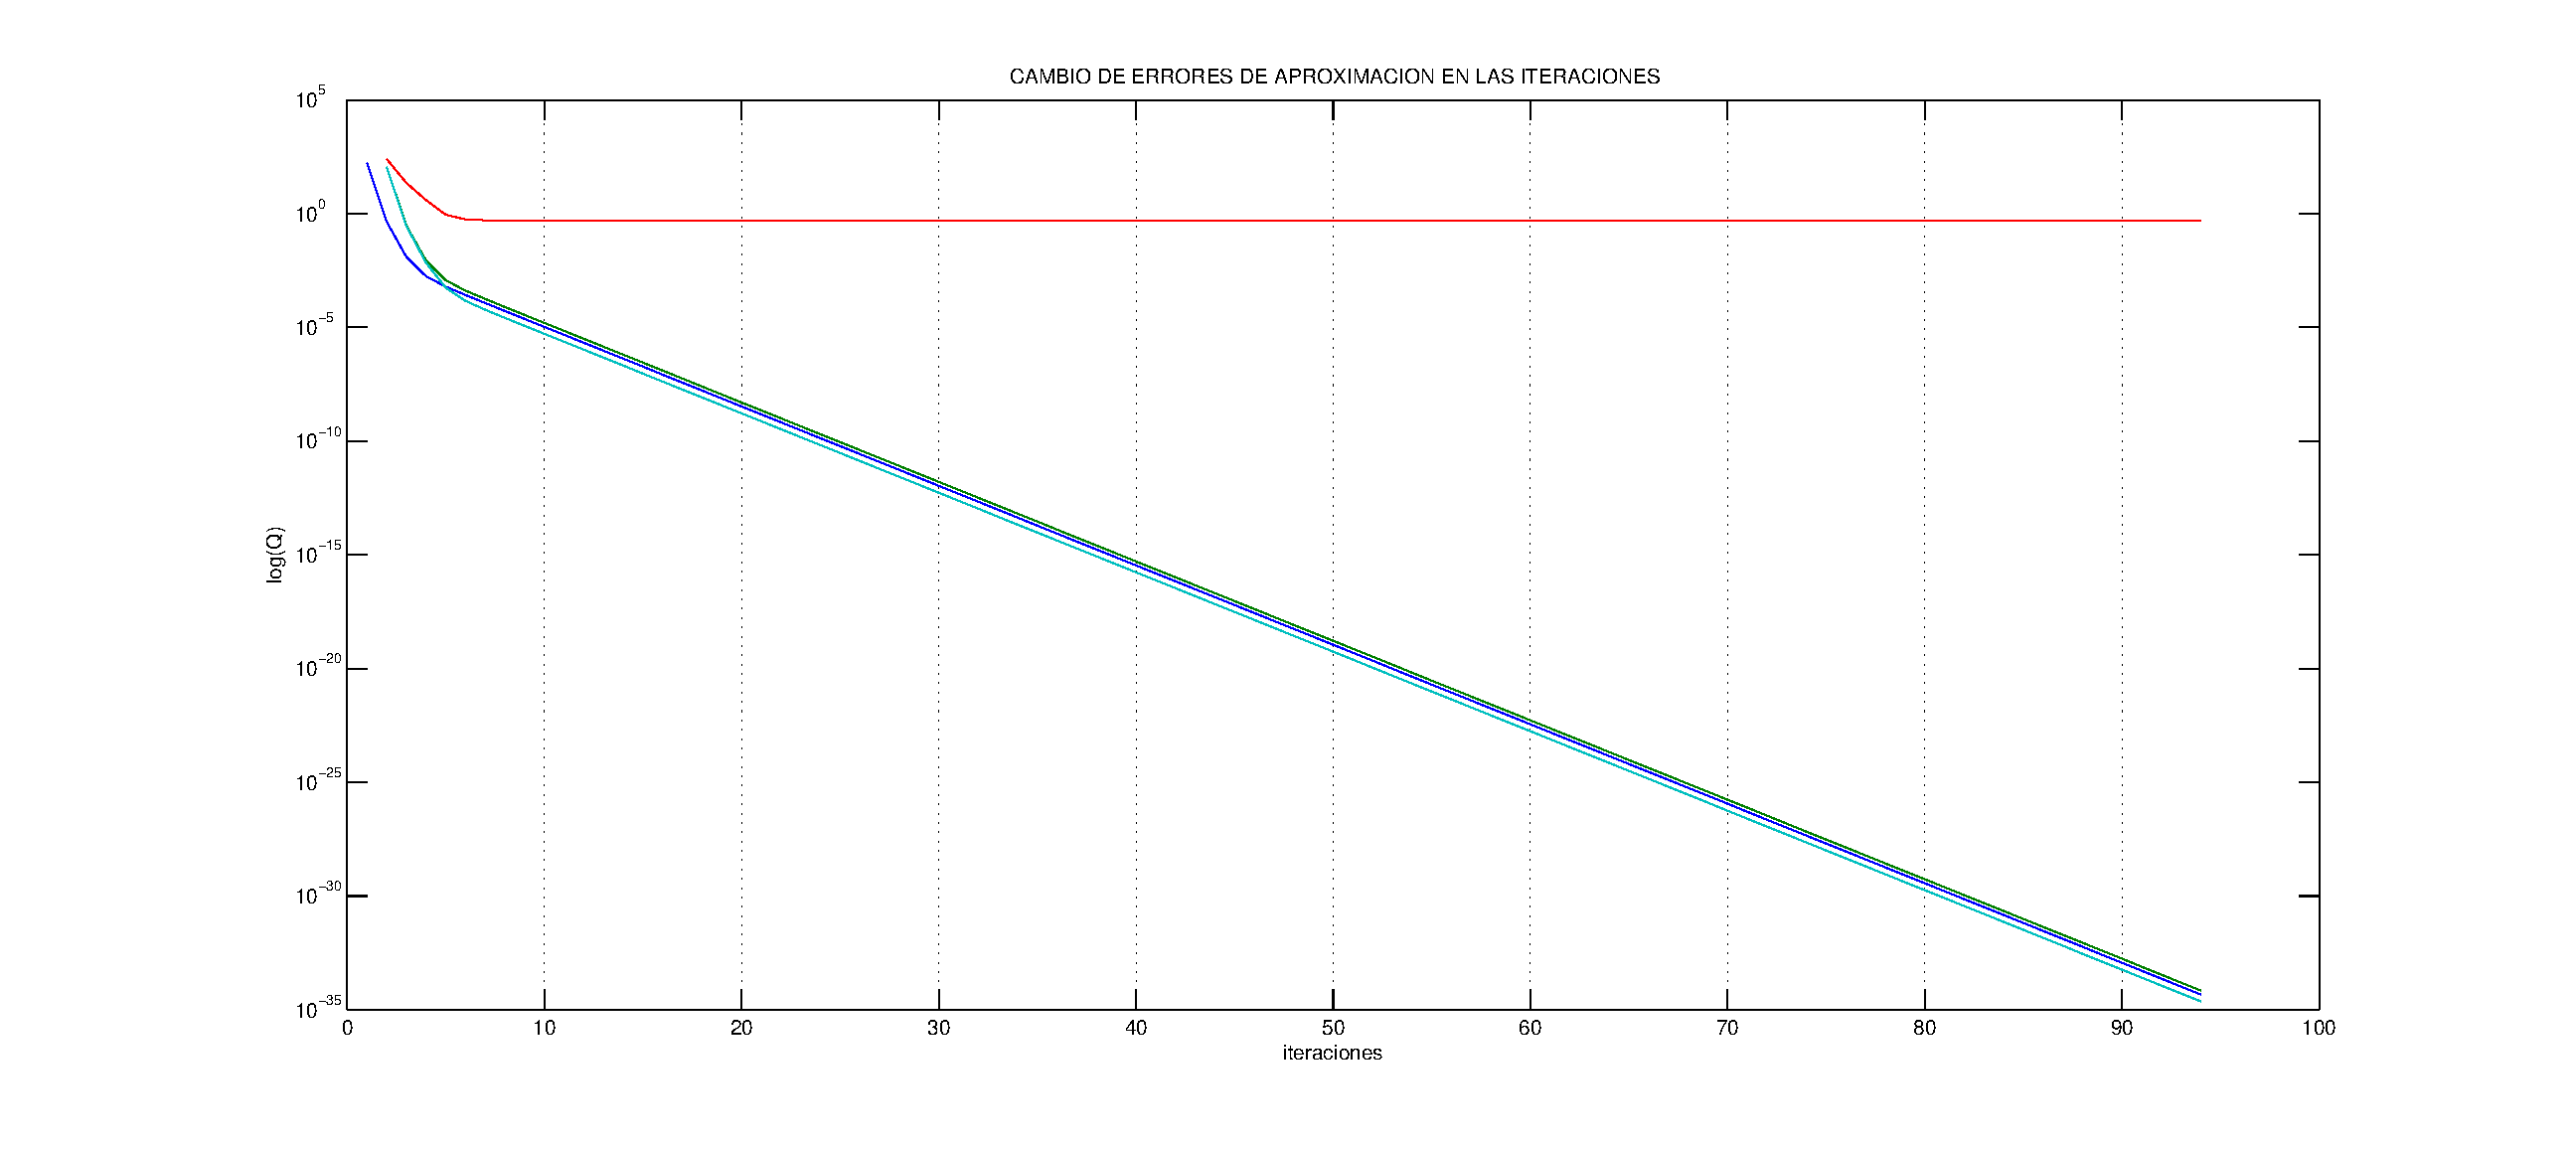
\includegraphics[scale=0.37]{Q1}
\noindent La gr\'afica muestra los cambios en $(d)$ logar\'itmos de valores diferentes a trav\'es de las iteraciones. Se utilizaron logaritmos de los valores para poder entender mejor la gr\'afica dado que los cambios entre los errores de aproximaci\'on (casi desde el principio de las iteraciones) son m\'inimo de $O(1/k^2)$
\begin{itemize}
\item Las curvas morado y verde representan al error absoluto de la aproximaci\'on, al tiempo k y al tiempo k+1, al cuadrado: $||x_k - x^*||_H^2$ .
\item La curva azul claro representa la diferencia absoluta entre el lado derecho de la desigualdad y el lado izquierdo, es decir, $LD - LI$.
\item Parece ser que la curva m\'as interesante es la roja, \'esta representa la diferencia relativa entre el lado derecho y el lado izquierdo, es decir, $(LD - LI) / LD$.
\par
\noindent Antes de analizar lo que esto puede significar, se expondr\'a la misma gr\'afica con los valores de los datos para la $5_a$ ejecuci\'on del programa ($N_{con} = 10^3$).\\
\\
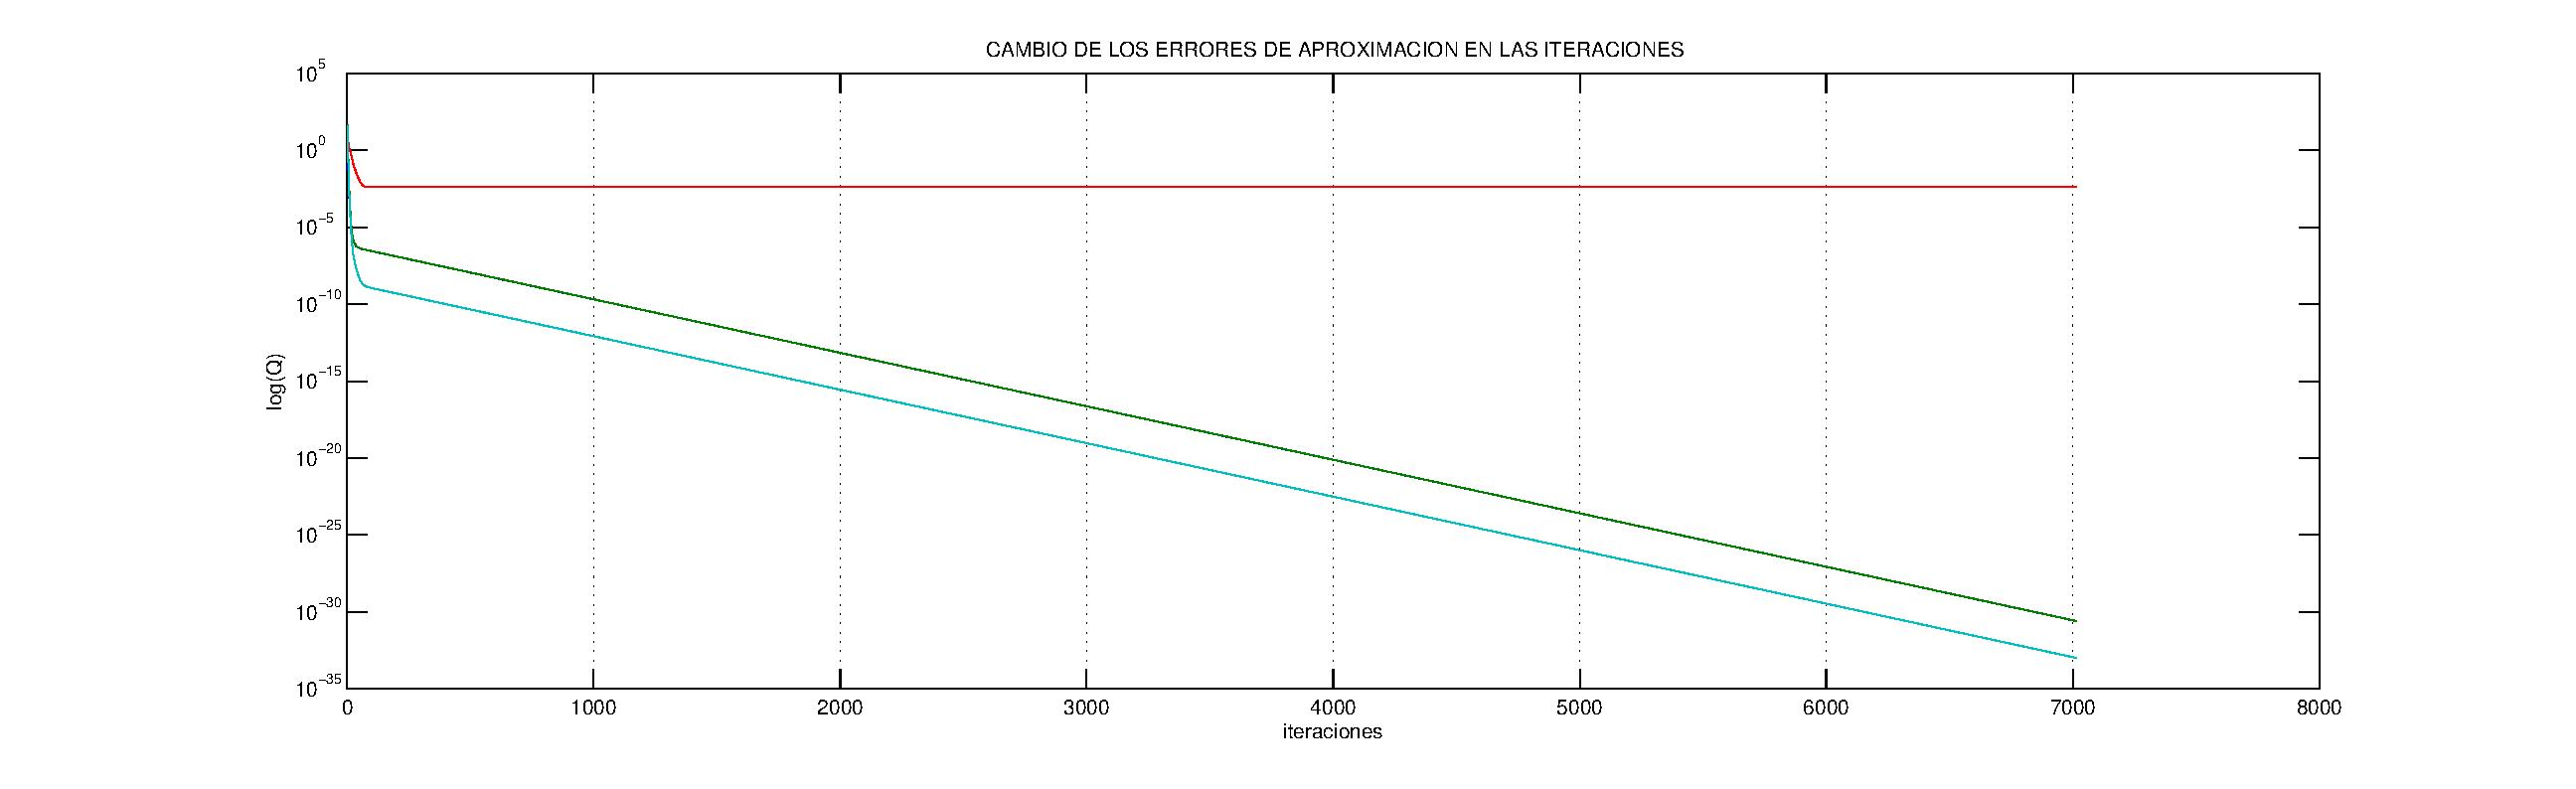
\includegraphics[trim = 40mm 0mm 40mm 0mm, clip, scale=.4]{Q2}
\item Las curvas de colores verde fuerte representan, de nuevo, los valores de el error absoluto de la aproximaci\'on al tiempo k.
\item La curva de color azul claro es el resultado de restar el lado derecho al lado izquierdo (diferencia absoluta).
\item La curva roja es la diferencia relativa entre los dos lados de la desigualdad.\\
\\
\noindent Si, bien, el n\'muero de iteraciones en $(e)$ crece (por el peor condicionamiento de la matriz), se puede notar el mismo comportamiento en los datos. Tanto los errores de aproximaci\'on como la diferencia absoluta (dos temas muy diferentes) decrecen de manera linear (en base al logaritmo de los datos). A\'un as\'i existe una diferencia mayor entre el lado izquierdo y el lado derecho para la segunda gr\'afica que para la primera, es decir, la distancia entre la l\'inea verde y la azul es mayor que entre la l\'inea morada y la azul. Esto podr\'ia explicarse porque la manera de acotar es diferente en los dos casos, depende de $cond(H)$. Sin embargo, lo que parece m\'as interesante de las dos gr\'afinas es como la diferencia relativa entre lado derecho y lado izquierdo parece estancarse en vez de seguir decreciendo. Al analizar los n\'meros que estas gr\'aficas arrojan, se ve la fuerza del condicionamiento de la matriz en ambos casos. Tanto el valor al que converge la diferencia relativa como la rapidez con la que lo hace es diferente en los dos casos. Para la matriz mejor condicionada, esta convergencia aparece casi de inmediato, adem\'as de que el valor al que lo hace es menor que en la matriz peor condicionada.
\\
\noindent Entonces, respondiendo la pregunta de si el lado izquierdo y el derecho son iguales, la respuesta ser\'ia que no, pero que , dependiendo de los valores propios de la matriz, se podr\'ia hacer un argumento en cuanto a su convergencia.\\
\end{itemize}
\item Prueba
\\
\indent Reconstrucci\'on de la prueba de Leunberger justificando.
 \\
 \\        
  \end{enumerate}
  
	
\subsubsection*{{\large Conclusiones}}
  \subsubsection*{ Tablas}

 \begin{table}[H]	
 	 \centering
  	  \caption{  \tt $N_o$. condici\'on = $10^1$   \hfill\small $(a)$}
    \begin{tabular}{|c|c|c|c|}
    \hline
    $k$     & $f_k$  & $||\nabla f_k||$ & $\alpha_k$ \\
    \hline
    1     & -7.1720741 & 1.21E+00 & 1.53E+00 \\
    2     & -8.6990872 & 9.78E-01 & 2.08E+00 \\
    4     & -9.9450389 & 6.24E-01 & 2.09E+00 \\
    30    & -10.873992 & 3.02E-03 & 2.09E+00 \\
    \hline
    \end{tabular}%
  \label{tab:$10^1$}%
\end{table}%

\begin{table}[htbp]
  \centering
  \caption*{\small resultados $1_a$ ejecuci\'on}
    \begin{tabular}{|r|r|r|}
    \hline
    $k_{final}$     & $f_{final}$  & $||\nabla f_{final}||$  \\
    \hline
    103   & -10.874013 & 8.40E-10 \\
    \hline
    \end{tabular}%
  \label{tab:addlabel}%
\end{table}%


\begin{table}[H]
  \centering
  \caption{\tt $N_o$. condici\'on = $10^2$  \hfill\small  $(b)$}
    \begin{tabular}{|c|c|c|c|}
    \hline
    $k$     & $f_k$  & $||\nabla f_k||$ & $\alpha_k$ \\
    \hline
    1     & -10.085693 & 1.94E+00 & 2.06E+00 \\
    2     & -13.546051 & 1.62E+00 & 1.84E+00 \\
    3     & -16.059326 & 1.47E+00 & 1.92E+00 \\
    4     & -18.111677 & 1.34E+00 & 1.90E+00 \\
    6     & -21.447377 & 1.20E+00 & 1.93E+00 \\
    8     & -24.200737 & 1.12E+00 & 1.95E+00 \\
    10    & -26.610402 & 1.05E+00 & 1.95E+00 \\
    13    & -29.792113 & 9.95E-01 & 2.00E+00 \\
    17    & -33.434125 & 9.15E-01 & 2.00E+00 \\
    22    & -37.224506 & 8.19E-01 & 1.96E+00 \\
    28    & -40.874672 & 7.26E-01 & 1.96E+00 \\
    37    & -44.942445 & 6.13E-01 & 2.00E+00 \\
    51    & -48.967301 & 4.63E-01 & 2.00E+00 \\
    86    & -53.006247 & 2.28E-01 & 1.96E+00 \\
    604   & -54.327843 & 7.19E-06 & 1.96E+00 \\ \hline
    \end{tabular}%
  \label{tab:addlabel}%
\end{table}%

\begin{table}[htbp]
  \centering
  \caption*{\small resultados $2_a$ ejecuci\'on}
    \begin{tabular}{|r|r|r|}
      \hline    $k_{final}$    & $f_{final}$  & $||\nabla f_{final}||$  \\
    \hline
    1048  & -54.327843 & 1.00E-09 \\   \hline
    \end{tabular}%
  \label{tab:addlabel}%
\end{table}%


\begin{table}[H]
  \centering
  \caption{\tt $N_o$ de condici\'on = $10^3$   \hfill\small  $(c)$}
    \begin{tabular}{|c|c|c|c||c|c|c|c|}
    \hline
    $k$     & $f_k$  & $||\nabla f_k||$ & $\alpha_k$  & $k$     & $f_k$  & $||\nabla f_k||$ & $\alpha_k$ \\
    \hline
&----------&---------------------------------&-------------------------------&-------------------------&-------------------------------&-------------------------------&-------------------------------&-------------------------------& \\ 
&     100  &   1.06849100e-03            15  &   7.82612000e-04           1  &   5.41002300e-03    15  &   2.53617700e-03          12  &   9.43142000e-04           1  &   9.10477000e-04          12  &   6.42398000e-04          14  & \\ 
&     400  &   1.14820800e-03            36  &   3.64050000e-04           1  &   5.56980000e-03    36  &   5.41822700e-03          18  &   7.34001000e-04           1  &   1.90074900e-03          19  &   1.25707400e-03          22  & \\ 
&     900  &   2.92952400e-03            55  &   2.00584800e-03           1  &   6.74806000e-03    55  &   4.96502900e-03          25  &   7.84278000e-04           1  &   2.30550200e-03          27  &   2.63791000e-03          29  & \\ 
&    1600  &   2.89594300e-03            72  &   3.02090600e-03           1  &   1.01153120e-02    72  &   6.98751200e-03          32  &   8.85159000e-04           1  &   4.40711900e-03          34  &   4.90156900e-03          36  & \\ 
&    2500  &   4.42903900e-03            88  &   1.39036050e-02           1  &   2.57833930e-02    88  &   1.29465660e-02          39  &   1.11018100e-03           1  &   1.32298600e-02          41  &   7.91524800e-03          41  & \\ 
&    3600  &   8.38852100e-03           105  &   1.39060120e-02           1  &   3.23225880e-02   105  &   1.73336430e-02          46  &   1.53305500e-03           1  &   1.34407480e-02          47  &   1.40587530e-02          46  & \\ 
&    4900  &   1.14804530e-02           121  &   2.16255590e-02           1  &   4.54670270e-02   121  &   2.43756310e-02          53  &   1.44365000e-03           1  &   1.95886370e-02          54  &   1.85902260e-02          51  & \\ 
&    6400  &   1.60968950e-02           138  &   3.05627350e-02           1  &   6.99073250e-02   138  &   3.30023130e-02          59  &   1.70702600e-03           1  &   3.30081160e-02          61  &   2.58359920e-02          55  & \\ 
&    8100  &   2.04724460e-02           155  &   4.54375290e-02           1  &   8.31877560e-02   155  &   4.45603520e-02          66  &   2.10226700e-03           1  &   3.89283530e-02          67  &   4.36928680e-02          60  & \\ 
&   10000  &   2.69440260e-02           172  &   6.87076140e-02           1  &   1.17569445e-01   172  &   1.14505605e-01          71  &   2.49615300e-03           1  &   5.51215140e-02          74  &   6.40166510e-02          65  & \\ 
&   12100  &   3.94897440e-02           188  &   8.83789180e-02           1  &   1.68043700e-01   188  &   8.28011660e-02          77  &   2.71815000e-03           1  &   7.93149730e-02          80  &   6.58539910e-02          68  & \\ 
&   14400  &   4.33175720e-02           205  &   1.17222861e-01           1  &   2.01051198e-01   205  &   1.11475609e-01          83  &   3.09578700e-03           1  &   9.29120490e-02          87  &   7.54882590e-02          72  & \\ 
&   16900  &   5.82257360e-02           221  &   1.46038922e-01           1  &   2.43268645e-01   221  &   1.38413102e-01          89  &   4.22672400e-03           1  &   1.20961235e-01          93  &   1.00767135e-01          76  & \\ 
&   19600  &   7.04430190e-02           238  &   1.79589695e-01           1  &   2.96194135e-01   238  &   1.53795593e-01          95  &   7.13745900e-03           1  &   1.65796609e-01          99  &   1.36001937e-01          80  & \\ 
&   22500  &   8.79010770e-02           254  &   2.60730149e-01           1  &   4.02322251e-01   254  &   2.05946315e-01         100  &   7.79754500e-03           1  &   1.88289730e-01         105  &   1.51452022e-01          83  & \\ 
&   25600  &   1.18728275e-01           271  &   2.93224254e-01           1  &   4.53904930e-01   271  &   3.00400033e-01         105  &   1.82403110e-02           1  &   2.32707991e-01         111  &   3.45642956e-01          86  & \\ 
&   28900  &   2.47618419e-01           287  &   4.05738646e-01           1  &   6.20211298e-01   287  &   2.61280932e-01         102  &   1.04726900e-02           1  &   2.99442658e-01         116  &   2.40565928e-01          89  & \\ 
&   32400  &   1.83634841e-01           304  &   3.97901999e-01           1  &   7.07080713e-01   304  &   3.10979257e-01         107  &   1.21899400e-02           1  &   3.64152655e-01         121  &   3.18325831e-01          92  & \\ 
&   36100  &   1.89486037e-01           320  &   4.44973987e-01           1  &   7.53485133e-01   320  &   3.29530477e-01         113  &   1.31811120e-02           1  &   3.75043467e-01         127  &   2.99734550e-01          96  & \\ 
&   40000  &   2.45583080e-01           336  &   5.76102487e-01           1  &   8.93528656e-01   336  &   4.18536002e-01         118  &   9.74169200e-03           1  &   4.57807157e-01         133  &   3.34086297e-01          99  & \\ 
&   44100  &   3.00589376e-01           353  &   5.90412097e-01           1  &   1.08363923e+00   353  &   4.81622338e-01         124  &   2.10367450e-02           1  &   5.01849485e-01         138  &   4.33093643e-01         101  & \\ 
&   48400  &   3.33143415e-01           369  &   6.91929033e-01           1  &   1.22339374e+00   369  &   5.38541071e-01         129  &   1.85215130e-02           1  &   5.75448164e-01         143  &   4.66470594e-01         105  & \\ 
&   52900  &   3.57908320e-01           385  &   8.59836239e-01           1  &   1.39623353e+00   385  &   6.15093294e-01         134  &   2.48203750e-02           1  &   6.96129542e-01         148  &   5.78907951e-01         107  & \\ 
&   57600  &   4.26533121e-01           402  &   9.30455629e-01           1  &   1.52442859e+00   402  &   6.98438086e-01         136  &   2.36627650e-02           1  &   7.43601591e-01         154  &   5.39497644e-01         110  & \\ 
&   62500  &   5.20005009e-01           418  &   1.15084217e+00           1  &   1.80969117e+00   418  &   7.39550753e-01         140  &   2.21715840e-02           1  &   8.30602294e-01         160  &   6.36120463e-01         113  & \\ 
&   67600  &   5.26979801e-01           434  &   1.27776959e+00           1  &   1.98538036e+00   434  &   8.17429527e-01         145  &   1.60215090e-02           1  &   1.14338694e+00         166  &   6.55749279e-01         116  & \\ 
&   72900  &   6.21803865e-01           450  &   1.43879309e+00           1  &   2.18759768e+00   450  &   9.08522911e-01         150  &   1.79581360e-02           1  &   1.30672305e+00         172  &   7.32951012e-01         118  & \\ 
&   78400  &   6.91826270e-01           466  &   1.57761600e+00           1  &   2.83274207e+00   466  &   1.01582917e+00         155  &   1.88924580e-02           1  &   1.58562660e+00         178  &   8.65604980e-01         120  & \\ 
&   84100  &   7.20860700e-01           483  &   1.87415391e+00           1  &   3.04612842e+00   483  &   1.15214747e+00         160  &   2.17907690e-02           1  &   1.60988093e+00         184  &   9.89255179e-01         123  & \\ 
&   90000  &   8.87573876e-01           498  &   2.11985762e+00           1  &   2.99012015e+00   498  &   1.22915163e+00         166  &   2.81576040e-02           1  &   1.86916465e+00         189  &   1.06627860e+00         125  & \\ 
&   96100  &   9.69454667e-01           515  &   2.34374369e+00           1  &   3.37384685e+00   515  &   1.28495613e+00         171  &   2.75052840e-02           1  &   1.95142044e+00         195  &   1.13575922e+00         128  & \\ 
&  102400  &   9.39550363e-01           531  &   2.95675079e+00           1  &   3.87800080e+00   531  &   1.44427702e+00         176  &   2.31211920e-02           1  &   2.13867667e+00         201  &   1.21034728e+00         131  & \\ 
&  108900  &   1.06053073e+00           547  &   2.66861660e+00           1  &   3.88059603e+00   547  &   1.59561129e+00         181  &   2.57185970e-02           1  &   2.28210681e+00         199  &   1.35077109e+00         134  & \\ 
&  115600  &   1.12314854e+00           563  &   3.37545122e+00           1  &   4.73342601e+00   563  &   1.92633519e+00         187  &   2.67743280e-02           1  &   2.54937088e+00         203  &   1.42924036e+00         135  & \\ 
&  122500  &   1.60492432e+00           579  &   3.74957665e+00           1  &   5.18994692e+00   579  &   1.87527933e+00         192  &   2.82590190e-02           1  &   2.48244463e+00         209  &   1.65179111e+00         138  & \\ 
&  129600  &   1.30840435e+00           596  &   3.43970660e+00           1  &   5.09743315e+00   596  &   2.02534213e+00         197  &   2.88596180e-02           1  &   2.63161608e+00         200  &   1.83726206e+00         140  & \\ 
&  136900  &   1.47154895e+00           611  &   4.55211379e+00           1  &   6.35100915e+00   611  &   2.23456634e+00         202  &   3.20929630e-02           1  &   3.11187166e+00         205  &   1.91901532e+00         142  & \\ 
&  144400  &   1.81437398e+00           627  &   4.34906978e+00           1  &   6.33031699e+00   627  &   2.40501081e+00         208  &   3.90787200e-02           1  &   2.93927452e+00         210  &   2.49558747e+00         145  & \\ 
&  152100  &   2.66728776e+00           644  &   6.34199663e+00           1  &   9.55660148e+00   644  &   3.60054661e+00         213  &   3.56026370e-02           1  &   3.70945876e+00         215  &   2.34747474e+00         147  & \\ 
&  160000  &   2.50055081e+00           659  &   6.34070456e+00           1  &   1.00697616e+01   659  &   3.02462980e+00         218  &   5.83746760e-02           1  &   3.93464665e+00         220  &   2.77079274e+00         149  & \\ 
&  168100  &   2.25408500e+00           675  &   6.70015363e+00           1  &   9.94769232e+00   675  &   2.90425958e+00         223  &   4.03754240e-02           1  &   3.82198809e+00         225  &   3.29299764e+00         152  & \\ 
&  176400  &   2.60017661e+00           692  &   7.77527341e+00           1  &   1.13033367e+01   692  &   3.15424966e+00         229  &   4.46870540e-02           1  &   5.48558084e+00         230  &   2.97726850e+00         153  & \\ 
&  184900  &   2.76257597e+00           707  &   9.44344938e+00           1  &   1.25035220e+01   707  &   3.72529037e+00         234  &   4.42049150e-02           1  &   4.88812346e+00         236  &   3.14401296e+00         156  & \\ 
&  193600  &   2.76753990e+00           724  &   7.71175208e+00           1  &   1.08901390e+01   724  &   3.66083670e+00         239  &   4.58042620e-02           1  &   4.53942152e+00         241  &   3.00239654e+00         158  & \\ 
&  202500  &   2.85210537e+00           739  &   8.67340172e+00           1  &   1.17601428e+01   739  &   3.83834713e+00         244  &   5.11065180e-02           1  &   4.77119160e+00         246  &   3.13765318e+00         161  & \\ 
&  211600  &   2.98907303e+00           755  &   9.43800387e+00           1  &   1.31692395e+01   755  &   4.20438817e+00         249  &   5.18954320e-02           1  &   5.24027078e+00         251  &   3.42375830e+00         163  & \\ 
&  220900  &   4.31323676e+00           771  &   9.97848479e+00           1  &   1.35663213e+01   771  &   4.44764493e+00         255  &   5.55841600e-02           1  &   5.65054687e+00         256  &   4.00247761e+00         165  & \\ 
&  230400  &   4.80647922e+00           787  &   1.22780637e+01           1  &   1.60832402e+01   787  &   4.65719652e+00         260  &   5.31996580e-02           1  &   6.54319365e+00         262  &   3.77327971e+00         167  & \\ 
&  240100  &   4.86274524e+00           803  &   1.21713788e+01           1  &   1.70287114e+01   803  &   4.99026828e+00         265  &   5.55263420e-02           1  &   7.50572062e+00         267  &   4.09684336e+00         169  & \\ 
&  250000  &   5.55551611e+00           818  &   1.36568578e+01           1  &   1.80061368e+01   818  &   5.79221089e+00         270  &   5.86349960e-02           1  &   7.43050586e+00         272  &   4.25660735e+00         170  & \\ 
    \hline
    \end{tabular}%
  \label{tab:addlabel}%
\end{table}%

\begin{table}[htbp]
  \centering
  \caption*{\small resultados $3_a$ ejecuci\'on}
    \begin{tabular}{|r|r|r|}
    \hline
      \hline    $k_{final}$    & $f_{final}$  & $||\nabla f_{final}||$  \\
    \hline
    9884  & -437.38824 & 9.99E-10 \\
    \hline
    \end{tabular}%
  \label{tab:addlabel}%
\end{table}%


\begin{table}[H]
  \centering
  \caption{\tt$N_o$ de condici\'on = $10^1$ , $g=-H*e$   \hfill \small $(d)$ }
    \begin{tabular}{|c|c|c|c|}
    \hline
    $k$     & $f_k$  & $||\nabla f_k||$ & $\alpha_k$ \\
    \hline
    1     & -3.213243 & 6.53E-01 & 1.36E+00 \\
    4     & -3.5340241 & 6.72E-02 & 1.64E+00 \\
    \hline
    \end{tabular}%
  \label{tab:addlabel}%
\end{table}%

\begin{table}[htbp]
  \centering
  \caption*{\small resultados $4_a$ ejecuci\'on para $x^*=e$}
    \begin{tabular}{|r|r|r|}
    \hline
      \hline    $k_{final}$    & $f_{final}$  & $||\nabla f_{final}||$  \\
    \hline
    94    & -3.5463799 & 8.90E-10 \\
    \hline
    \end{tabular}%
  \label{tab:addlabel}%
\end{table}%


\begin{table}[H]
  \centering
   \caption{\tt$N_o$ de condici\'on = $10^3$ , $g=-H*e$   \hfill \small $(e)$ }
    \begin{tabular}{|r|r|r|r|}
    \hline
    $k$     & $f_k$  & $||\nabla f_k||$ & $\alpha_k$ \\
    \hline
    1     & -1.3115673 & 8.35E-01 & 1.44E+00 \\
    2     & -1.8557898 & 4.58E-01 & 1.56E+00 \\
    4     & -2.096884 & 2.02E-01 & 1.71E+00 \\
    401   & -2.1802517 & 5.58E-04 & 1.98E+00 \\
    3443  & -2.1803304 & 1.27E-06 & 1.98E+00 \\
    \hline
    \end{tabular}%
  \label{tab:addlabel}%
\end{table}%

\begin{table}[htbp]
  \centering
  \caption*{\small resultados $5_a$ ejecuci\'on para $x^*=e$}
    \begin{tabular}{|r|r|r|}
    \hline
      \hline    $k_{final}$    & $f_{final}$  & $||\nabla f_{final}||$  \\
    \hline
    7017  & -2.1803304 & 9.98E-10 \\
    \hline
    \end{tabular}%
  \label{tab:addlabel}%
\end{table}%


 
\end{document}